
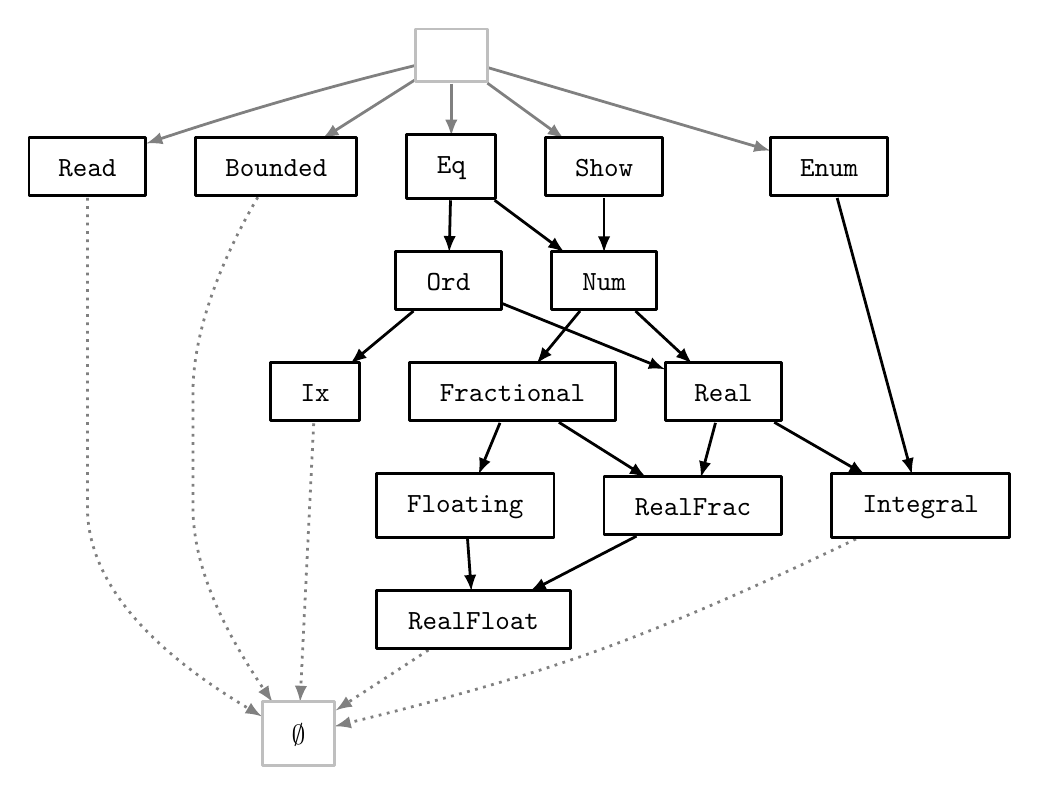
\begin{tikzpicture}[>=latex,line join=bevel,]
  \pgfsetlinewidth{1bp}
%%
\pgfsetcolor{black}
  % Edge: \texttt{Eq} -> \texttt{Num}
  \draw [->] (167.61bp,204.36bp) .. controls (172.91bp,200.42bp) and (178.92bp,195.93bp)  .. (192.67bp,185.69bp);
  % Edge: \texttt{Show} -> \texttt{Num}
  \draw [->] (207bp,205.23bp) .. controls (207bp,202.29bp) and (207bp,199bp)  .. (207bp,185.56bp);
  % Edge: \kindStar -> \texttt{Read}
  \pgfsetcolor{gray}
  \draw [->] (138.79bp,252.83bp) .. controls (120.95bp,248.45bp) and (88.037bp,240.01bp)  .. (42.198bp,224.81bp);
  % Edge: \kindStar -> \texttt{Enum}
  \draw [->] (165.04bp,252.16bp) .. controls (186.09bp,245.97bp) and (228.14bp,233.61bp)  .. (266.82bp,222.23bp);
  % Edge: \texttt{Ix} -> \emptyset
  \draw [->,dotted] (102.47bp,124.08bp) .. controls (101.48bp,103.92bp) and (99.364bp,60.469bp)  .. (97.575bp,23.787bp);
  % Edge: \kindStar -> \texttt{Show}
  \draw [->] (165.03bp,246.52bp) .. controls (170.71bp,242.39bp) and (177.54bp,237.42bp)  .. (192.51bp,226.54bp);
  % Edge: \texttt{Floating} -> \texttt{RealFloat}
  \pgfsetcolor{black}
  \draw [->] (157.85bp,82.361bp) .. controls (158.05bp,79.7bp) and (158.26bp,76.793bp)  .. (159.22bp,63.685bp);
  % Edge: \texttt{RealFloat} -> \emptyset
  \pgfsetcolor{gray}
  \draw [->,dotted] (143.78bp,42.441bp) .. controls (136.17bp,37.493bp) and (127bp,31.525bp)  .. (110.41bp,20.725bp);
  % Edge: \texttt{Fractional} -> \texttt{Floating}
  \pgfsetcolor{black}
  \draw [->] (169.53bp,124.23bp) .. controls (168.35bp,121.38bp) and (167.04bp,118.21bp)  .. (161.85bp,105.71bp);
  % Edge: \texttt{Num} -> \texttt{Fractional}
  \draw [->] (198.33bp,164.49bp) .. controls (195.55bp,161.12bp) and (192.38bp,157.28bp)  .. (182.73bp,145.58bp);
  % Edge: \kindStar -> \texttt{Eq}
  \pgfsetcolor{gray}
  \draw [->] (152bp,246.32bp) .. controls (152bp,243.67bp) and (152bp,240.7bp)  .. (152bp,227.59bp);
  % Edge: \texttt{Real} -> \texttt{Integral}
  \pgfsetcolor{black}
  \draw [->] (268.28bp,124.44bp) .. controls (275.57bp,120.24bp) and (284.13bp,115.29bp)  .. (301.03bp,105.53bp);
  % Edge: \texttt{Read} -> \emptyset
  \pgfsetcolor{gray}
  \draw [->,dotted] (21bp,205.26bp) .. controls (21bp,189.74bp) and (21bp,160.17bp)  .. (21bp,135bp) .. controls (21bp,135bp) and (21bp,135bp)  .. (21bp,94bp) .. controls (21bp,62.07bp) and (52.381bp,37.317bp)  .. (83.762bp,18.559bp);
  % Edge: \texttt{Enum} -> \texttt{Integral}
  \pgfsetcolor{black}
  \draw [->] (290.93bp,205.17bp) .. controls (296.36bp,185.08bp) and (308.1bp,141.69bp)  .. (317.84bp,105.69bp);
  % Edge: \texttt{Bounded} -> \emptyset
  \pgfsetcolor{gray}
  \draw [->,dotted] (82.342bp,205.46bp) .. controls (73.504bp,190.43bp) and (59bp,161.69bp)  .. (59bp,135bp) .. controls (59bp,135bp) and (59bp,135bp)  .. (59bp,94bp) .. controls (59bp,71.309bp) and (71.127bp,48.087bp)  .. (87.607bp,23.71bp);
  % Edge: \texttt{Ord} -> \texttt{Ix}
  \pgfsetcolor{black}
  \draw [->] (138.39bp,164.49bp) .. controls (133.8bp,160.66bp) and (128.48bp,156.23bp)  .. (115.69bp,145.58bp);
  % Edge: \texttt{Eq} -> \texttt{Ord}
  \draw [->] (151.72bp,204.36bp) .. controls (151.65bp,201.7bp) and (151.58bp,198.79bp)  .. (151.26bp,185.69bp);
  % Edge: \texttt{Ord} -> \texttt{Real}
  \draw [->] (170.09bp,167.29bp) .. controls (184.05bp,161.65bp) and (203.27bp,153.88bp)  .. (228.91bp,143.52bp);
  % Edge: \texttt{Num} -> \texttt{Real}
  \draw [->] (218.3bp,164.49bp) .. controls (222.22bp,160.84bp) and (226.72bp,156.65bp)  .. (238.63bp,145.58bp);
  % Edge: \texttt{Fractional} -> \texttt{RealFrac}
  \draw [->] (190.74bp,124.44bp) .. controls (197.66bp,120.08bp) and (205.84bp,114.92bp)  .. (222.09bp,104.67bp);
  % Edge: \texttt{Real} -> \texttt{RealFrac}
  \draw [->] (247.11bp,124.23bp) .. controls (246.3bp,121.19bp) and (245.38bp,117.78bp)  .. (241.83bp,104.56bp);
  % Edge: \texttt{Integral} -> \emptyset
  \pgfsetcolor{gray}
  \draw [->,dotted] (297.66bp,82.42bp) .. controls (274.33bp,71.137bp) and (237.25bp,53.979bp)  .. (204bp,42bp) .. controls (175.58bp,31.763bp) and (141.91bp,22.827bp)  .. (110.04bp,15.008bp);
  % Edge: \texttt{RealFrac} -> \texttt{RealFloat}
  \pgfsetcolor{black}
  \draw [->] (218.66bp,83.441bp) .. controls (209.72bp,78.803bp) and (199.05bp,73.268bp)  .. (180.28bp,63.523bp);
  % Edge: \kindStar -> \texttt{Bounded}
  \pgfsetcolor{gray}
  \draw [->] (138.95bp,247.71bp) .. controls (131.78bp,243.16bp) and (122.64bp,237.36bp)  .. (105.64bp,226.56bp);
  % Node: \texttt{Show}
\begin{scope}
  \definecolor{strokecol}{rgb}{0.0,0.0,0.0};
  \pgfsetstrokecolor{strokecol}
  \draw (228bp,227bp) -- (186bp,227bp) -- (186bp,206bp) -- (228bp,206bp) -- cycle;
  \draw (207bp,216bp) node {$\texttt{Show}$};
\end{scope}
  % Node: \texttt{Ord}
\begin{scope}
  \definecolor{strokecol}{rgb}{0.0,0.0,0.0};
  \pgfsetstrokecolor{strokecol}
  \draw (170bp,186bp) -- (132bp,186bp) -- (132bp,165bp) -- (170bp,165bp) -- cycle;
  \draw (151bp,175bp) node {$\texttt{Ord}$};
\end{scope}
  % Node: \texttt{Enum}
\begin{scope}
  \definecolor{strokecol}{rgb}{0.0,0.0,0.0};
  \pgfsetstrokecolor{strokecol}
  \draw (309bp,227bp) -- (267bp,227bp) -- (267bp,206bp) -- (309bp,206bp) -- cycle;
  \draw (288bp,216bp) node {$\texttt{Enum}$};
\end{scope}
  % Node: \texttt{Ix}
\begin{scope}
  \definecolor{strokecol}{rgb}{0.0,0.0,0.0};
  \pgfsetstrokecolor{strokecol}
  \draw (119bp,146bp) -- (87bp,146bp) -- (87bp,125bp) -- (119bp,125bp) -- cycle;
  \draw (103bp,135bp) node {$\texttt{Ix}$};
\end{scope}
  % Node: \texttt{Integral}
\begin{scope}
  \definecolor{strokecol}{rgb}{0.0,0.0,0.0};
  \pgfsetstrokecolor{strokecol}
  \draw (353bp,106bp) -- (289bp,106bp) -- (289bp,83bp) -- (353bp,83bp) -- cycle;
  \draw (321bp,94bp) node {$\texttt{Integral}$};
\end{scope}
  % Node: \texttt{Bounded}
\begin{scope}
  \definecolor{strokecol}{rgb}{0.0,0.0,0.0};
  \pgfsetstrokecolor{strokecol}
  \draw (118bp,227bp) -- (60bp,227bp) -- (60bp,206bp) -- (118bp,206bp) -- cycle;
  \draw (89bp,216bp) node {$\texttt{Bounded}$};
\end{scope}
  % Node: \kindStar
\begin{scope}
  \definecolor{strokecol}{rgb}{0.75,0.75,0.75};
  \pgfsetstrokecolor{strokecol}
  \draw (165bp,266bp) -- (139bp,266bp) -- (139bp,247bp) -- (165bp,247bp) -- cycle;
  \definecolor{strokecol}{rgb}{0.0,0.0,0.0};
  \pgfsetstrokecolor{strokecol}
  \draw (152bp,256bp) node {$\kindStar$};
\end{scope}
  % Node: \texttt{RealFloat}
\begin{scope}
  \definecolor{strokecol}{rgb}{0.0,0.0,0.0};
  \pgfsetstrokecolor{strokecol}
  \draw (195bp,64bp) -- (125bp,64bp) -- (125bp,43bp) -- (195bp,43bp) -- cycle;
  \draw (160bp,53bp) node {$\texttt{RealFloat}$};
\end{scope}
  % Node: \texttt{RealFrac}
\begin{scope}
  \definecolor{strokecol}{rgb}{0.0,0.0,0.0};
  \pgfsetstrokecolor{strokecol}
  \draw (271bp,105bp) -- (207bp,105bp) -- (207bp,84bp) -- (271bp,84bp) -- cycle;
  \draw (239bp,94bp) node {$\texttt{RealFrac}$};
\end{scope}
  % Node: \texttt{Fractional}
\begin{scope}
  \definecolor{strokecol}{rgb}{0.0,0.0,0.0};
  \pgfsetstrokecolor{strokecol}
  \draw (211bp,146bp) -- (137bp,146bp) -- (137bp,125bp) -- (211bp,125bp) -- cycle;
  \draw (174bp,135bp) node {$\texttt{Fractional}$};
\end{scope}
  % Node: \texttt{Floating}
\begin{scope}
  \definecolor{strokecol}{rgb}{0.0,0.0,0.0};
  \pgfsetstrokecolor{strokecol}
  \draw (189bp,106bp) -- (125bp,106bp) -- (125bp,83bp) -- (189bp,83bp) -- cycle;
  \draw (157bp,94bp) node {$\texttt{Floating}$};
\end{scope}
  % Node: \texttt{Real}
\begin{scope}
  \definecolor{strokecol}{rgb}{0.0,0.0,0.0};
  \pgfsetstrokecolor{strokecol}
  \draw (271bp,146bp) -- (229bp,146bp) -- (229bp,125bp) -- (271bp,125bp) -- cycle;
  \draw (250bp,135bp) node {$\texttt{Real}$};
\end{scope}
  % Node: \texttt{Num}
\begin{scope}
  \definecolor{strokecol}{rgb}{0.0,0.0,0.0};
  \pgfsetstrokecolor{strokecol}
  \draw (226bp,186bp) -- (188bp,186bp) -- (188bp,165bp) -- (226bp,165bp) -- cycle;
  \draw (207bp,175bp) node {$\texttt{Num}$};
\end{scope}
  % Node: \emptyset
\begin{scope}
  \definecolor{strokecol}{rgb}{0.75,0.75,0.75};
  \pgfsetstrokecolor{strokecol}
  \draw (110bp,24bp) -- (84bp,24bp) -- (84bp,1bp) -- (110bp,1bp) -- cycle;
  \definecolor{strokecol}{rgb}{0.0,0.0,0.0};
  \pgfsetstrokecolor{strokecol}
  \draw (97bp,12bp) node {$\emptyset$};
\end{scope}
  % Node: \texttt{Eq}
\begin{scope}
  \definecolor{strokecol}{rgb}{0.0,0.0,0.0};
  \pgfsetstrokecolor{strokecol}
  \draw (168bp,228bp) -- (136bp,228bp) -- (136bp,205bp) -- (168bp,205bp) -- cycle;
  \draw (152bp,216bp) node {$\texttt{Eq}$};
\end{scope}
  % Node: \texttt{Read}
\begin{scope}
  \definecolor{strokecol}{rgb}{0.0,0.0,0.0};
  \pgfsetstrokecolor{strokecol}
  \draw (42bp,227bp) -- (0bp,227bp) -- (0bp,206bp) -- (42bp,206bp) -- cycle;
  \draw (21bp,216bp) node {$\texttt{Read}$};
\end{scope}
%
\end{tikzpicture}

